\section{Object Oriented Design}
    Object orientated programming is a very powerful concept but does not always lead to quality
    software. There are 5 principles that focus on dependency management to avoid code that
    is breakable, fragile and hard to maintain. This is why the SOLID \cite{Hotop2015} 
    principles of OOP should be applied.
    SOLID stands for :
    \begin{enumerate}
        \item 
            \textbf{S}ingle Responsibility Principle
        \item 
            \textbf{O}pen Closed Principle
        \item 
            \textbf{L}iskov Substitution Principle
        \item 
            \textbf{I}nterface Segregation Principle
        \item 
            \textbf{D}ependency Inversion Principle
    \end{enumerate}

    \subsection{SOLID Design}
        In this section, I would like to describe in detail how the SOLID principles will 
        be designed in the navigation module.
       \subsubsection{Single Responsibility Principle}
        This principle states that there every class should have a single responsibility
        and there should never be more than one reason to change the class. 
        The code base is sub divided in to 8 packages so that the  and they are:
        \newpage
        \begin{enumerate}
            \item 
                \textbf{constants} 
                    this package contains constants like the Raspberry pi pin 
                    numbers, API endpoints. All the variable which will not 
                    change and could be used in the project are normally kept here.
            \item 
                \textbf{presenters} 
                    This package contains the presenters for the model and the view.
                    The class Navigation Manager is here which is responsible to communicate
                    with the view and all the three services (I/O service, GPS service and 
                    Direction API Service).  
            \item 
                \textbf{customExceptions}
                    This package would contain custom exceptions if created.
            \item 
                \textbf{Interfaces}
                    This package contains all the Interfaces for the corresponding classes. 
            \item 
                \textbf{listners}
                    This package contains custom asynchronous android listeners which gets 
                    called when the task get done. For example a listener to get the result
                    from the google API server is also here. 
            \item 
                \textbf{models}
                This package contains the data layers mainly 
                \href{https://spring.io/understanding/POJO}  {POJO}. Classes defining how the
                data should look like.
            \item 
                \textbf{services} 
                    This packages consist of sub packages for the I/O, GPS and Direction service.
            \item 
                \textbf{utils}
                    This package has the utilities for making the API requests and other utilities. 
        \end{enumerate}

        \par
            % Write about why I decided about the two classes and how single responsibility is behind this decision  \ref{fig:directionServiceClassDiagram} 
        \begin{figure}[htbp!]
            \centering 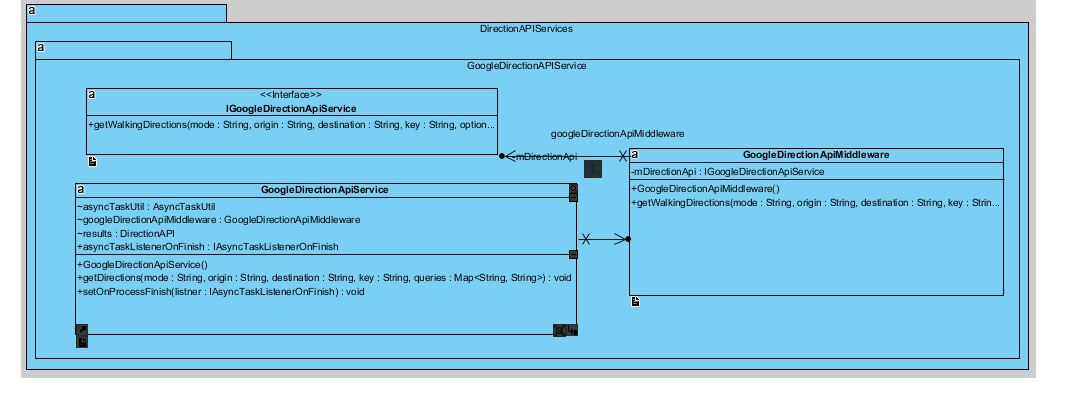
\includegraphics[scale=0.6]{grafiken/directionService.jpg}
            \caption{Class Diagram: Design of the Direction API service}
            \label{fig:directionServiceClassDiagram}
        \end{figure}